\graphicspath{{chapters/images/cf_mg/}}
\chapter{CFPS and MAGE}
\section{Cell-free protein synthesis}
Cell-free protein synthesis is also called IVVT (in vitro transcription translation). 
We take living cells, grow them up to a certain density, lyse the membrane to get the cytoplasm and use it to run a metabolic reaction.
CFPS can be defined as the production of proteins using biological machinery without the use of living cells. 
The in-vitro protein synthesis environment is not constrained by a cell wall or homeostasis conditions necessary to maintain cell viability. 
CFPS enables direct access and control of the translation environment, which is advantageous for a number of applications including: optimization of protein production, optimization of protein complexes, study of protein synthesis, incorporating non-natural amino acids, high-throughput screens, and synthetic biology.
For instance,  incorporating non natural amino acids could be poisonous for the cell,  but in this case this can be performed - as the cell is not viable anymore. 
George Curch is one of the pioneers in the field. He states the following advantages of CFPS:
\begin{enumerate}
	\item rather than attempt to balance the tug-of- war between the cell’s objectives and the engineer’s objectives, in vitro biocatalysis focuses cellular resources toward an exclusive user-defined objectives. 
	\item cell viability constraints are removed. 
	\item transport barriers are removed, allowing easy substrate addition, product removal, system monitoring, and rapid sampling. 
\end{enumerate}
\noindent
There are two main CFPS types: 
\begin{itemize}
	\item Cell extract: grow cell population, disrupt the membrane and isolate the metabolism hoping that the proteins are still viable. We have four major sources for extraction: Escherichia coli (ECE), rabbit reticulocytes (RRL), wheat germ (WGE), insect cells (ICE). We choose according to the kind of protein we are interested in, as protein production in E. coli and eukaryotes is quite different.
All of these extracts are commercially available. 
	\item The PURE system (E.coli only). Individual compotents for transcription machinery are isolated.
\end{itemize}

\noindent
CFPS is quite important (remember tocopherol from Lecture 1). In 1960s it was not clear how to map DNA information to protein production. Nirenberg was the first to find the first codon sequence – UUU, phenylalanine. 

\subsection{Cell extract}
\begin{figure}[h]
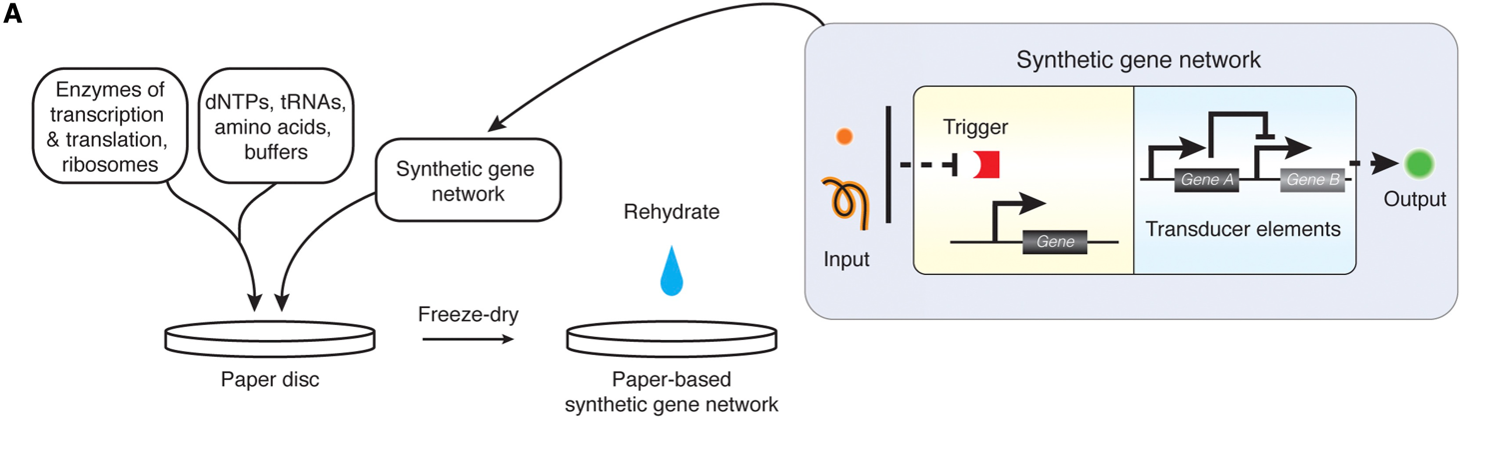
\includegraphics[width=1\textwidth]{cfps}
\caption{\label{fig:cfps} Cell-free protein synthesis procedure}
\end{figure}

\noindent
The cell extract is put on a paper filter disc with basic components (dNTPs, tRNAs) and freexe-dryed. The disk is rehydrated, hoping that functions are restored. If the synthetic gene network is active, we should get a tangible output. The same can be applied with plasmid DNA or inducers, we can check GFP expression. We get everything that the cell produces, also potential dangers e.g. proteases, lysosomes.

\subsection{PURE system}
The PURE system (Protein synthesis Using Recombinant Elements) is the reconstitution the E.coli (transcription) translation process in a test tube. It provides higher reaction controllability in comparison to crude cell-free protein- synthesis systems for translation studies and biotechnology applications. 
The PURE system stands out among translation methods in that it provides not only a simple and unique “reverse” purification method of separating the synthesized protein from reaction mixture, but also that the system can be tailor-made according to individual protein requirements.” 

\begin{figure}
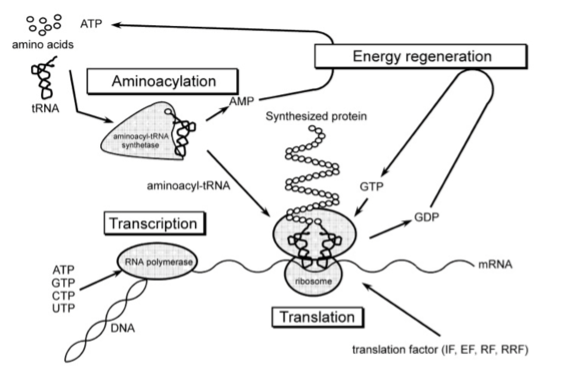
\includegraphics[width=0.5\textwidth, center ]{pure}
\caption{\label{fig:pure} PURE procedure}
\end{figure}
\noindent
Required materials are RNA polymerase, monomers, ribosome, tRNAs (aminoacylation), we require energy for reactions (ATP, GTP …). 
We also need all the enzymes e.g. kinases, phosphate economy control. 
The system needs to be buffered and protected from oxidation (DTT is used to avoid this), pH control is required to avoid unwanted molecular interactions and protein folding, light should be also controlled. Everything has to be purified and reconstituted. 
It was possible to make with a good range of proteins; control is good, we can fully customize the system. The tradeoff is that we get a small protein yield with respect to other techniques. 
DNA is prepared for PCR with a FOR and REV primer + specific promoter. The ribosomes are supplied intact (avoid complex assembly).
\\
\\
\noindent
Advantages over cell-free extract: because its components are defined, the PURE system does not contain some detrimental enzymes found in extracts. Individual components can be varied, added or subtracted depending in the application.  PUREfrex Technology allows to obtain proteins for antibody generation, structural and kinetic studies and screening assays.
\\
\\
\noindent
This system is good at making proteins from a gene, but not a replication (instead this occurs in a flow reactor). We have to keep feeding the system with the required materials, which are very expensive - not economically practical, everything is done in batch mode.
Reducing a complex system will lead lacking the optimal yield, but ensuring good quality. The cell is maintaining concentrations of metabolites and proteins in a smart way, in this case instead we lose  control. Glycosylation is an important process to take into consideration, involved in regulation.

\section{Multiplex Automated Genome Engineering}
The aim of MAGE is to improve changes in the genome (insertion/deletions) at specific positions. DNA replication occurs in section, the DNA is un-winded and the RNA polymerase starts from the leading strand (5’ to 3’ direction), then on the lagging strand from Okazaki fragments. We can overwhelm the system by adding artificial fragments, which should be similar to the wild type to create competition thermodynamics drives the process.
\\
\\
\noindent
The efficiency of the MAGE process was characterized using a modified E. coli strain, mediated by a bacteriophage ssDNA-binding protein beta. The beta protein directs ssDNA to the lagging strand and promotes strand annealing. This strain also lacks mismatch repair. Sometimes the competition does not work, we have different outcomes. The oligos can be different e.g. ssDNA oligo, substitutions… The flanking regions must be faithful to ensure a correct recognition.
Linear DNA molecules are flanked by homologous sequences (40-50 bp are more efficient) to target DNA sequences (1-60 nt). It is possible to insert N variations in the case in which it is not sure which modification to make. Each site can have variation and its own pool of oligos, massively parallel gene editing process.
\\
\\
\noindent
Process: grow cells until a certain density is reached, include ss-oligos and obtain replacement by electroporation. Some cells do not survive electroporation, some do not take up external DNA, some take some oligos and get genetically modified. After some recovery time, cells are grown again and the process is repeated. At any time, it is possible to harvest some cells for screening, selection or genotyping. 
\\
\\
\noindent
For each cycle, a certain percentage of population is genetically modified. To overcome low efficiency, the oligo-recombineering protocol is iterated on the same cell population over multiple cycles using the same oligo species. In this fashion, the population is enriched for mutants containing the desired sequence conversions. Each full cycle takes 2-3 h, depending on the growth rate of the cells. 
\\
\\
\noindent
The relative abundance of mutants in the population $M$ can be approximated by $M=1-(1-RE)^N$ where $N$ is the number of cycles and $RE$ is the allelic replacement efficiency per cycle. 
$RE$ is highly dependent on the type of target conversion (mismatch, insertion, deletion) and the size of the conversion. 
The efficiency depends on the amount of genetic modification we wish to add (figure), as it becomes increasingly difficul for fragments to compete when they diverge from the original sequence.
\begin{figure}
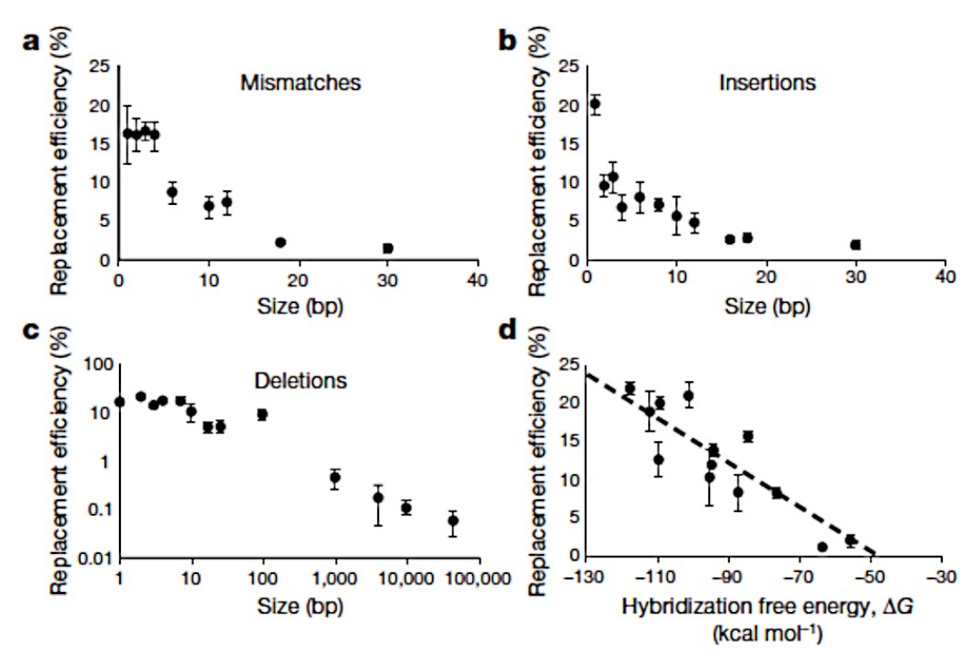
\includegraphics[width=0.5\textwidth, center ]{rep_eff}
\caption{\label{fig:rep_eff} Replacement efficiency in mismatches, insertions, deletions}
\end{figure}
\\
\\
\noindent
Genetic screens can be in the form of direct genotypic methods such as PCR or DNA sequencing, or phenotypic screening or selection methods such as colorimetry, growth rate, or antibiotic resistance. 
By computing $N=$, we can find the number of cycles $N$ needed to produce mutation size of b base-pairs at a frequency of at least F in the population.
For example, the number of cycles needed to generate mutants with a 6 bp chromosomal mismatch to a frequency of 0.25 (i.e., 25\%) in the population with an oligo folding energy of - 5.4 kcal/mol (predicted through MFold; Markham and Zuker, 2005) is $N=log(1-0.25)/log(1-0.26x e^-0.135 x 5)=2.0$ cycles, and to a frequency of 0.50 (i.e., 50\%) is $N = 4.9$ cycles. 
Thus, one would expect from a PCR screen that at least one in four cells would show conversion after two cycles and one in two would show conversion after five cycles of oligo-recombineering. 
This frequency is high enough that alterations can now be made without selection. With optimized protocols, over 50\% of the cells that survive electroporation contain the desired change. 
\\
\\
\noindent
Multiple cyclings with multiple targets can lead to a combinatorial explosion with the main limitation being the cell population size (around $10^9$ cells). 
MAGE test system: the targeted lacZ region was sequenced in 96 random clonal isolates after MAGE cycles 2,5,10 and 15 that provided a snapshot of the genotypic variation in each population.   
We have consecutive N30 oligo, insterspered n6 oligo and consecutive N6.  While cycles increase, we see an increase in mutations.
\begin{figure}
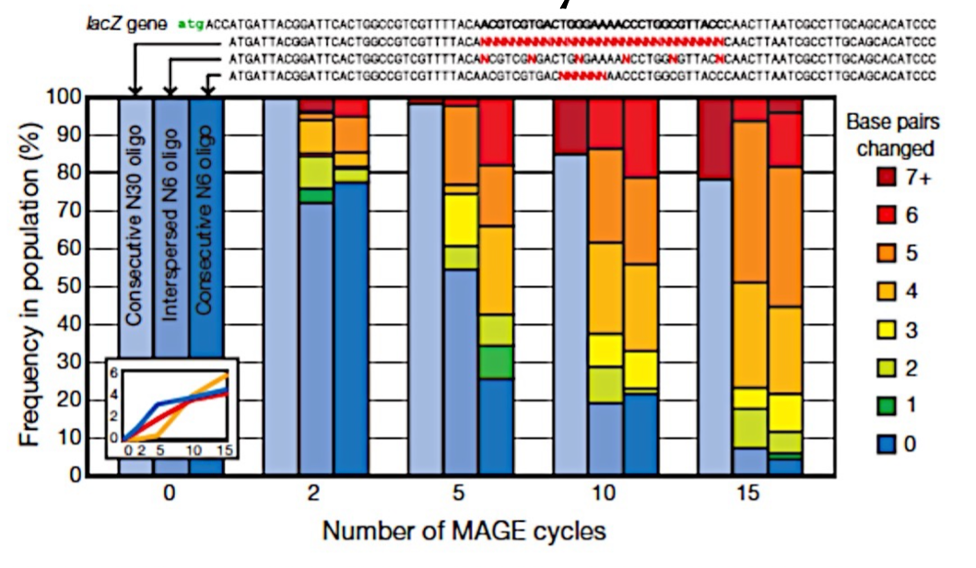
\includegraphics[width=0.5\textwidth, center ]{mage_test}
\caption{\label{fig:mage_test} Sequence diversity generated across three separate cell populations as a function of the number of MAGE cycles}
\end{figure}
\noindent
The depth at which MAGE generates diversity is determined by a combination of three factors: 
\begin{enumerate}
	\item the degree of sequence variation desired at each locus; 
	\item the number of loci targeted; 
	\item the number of MAGE cycles performed. 
\end{enumerate}
\noindent
\subsection{MAGE automation}

\begin{figure}
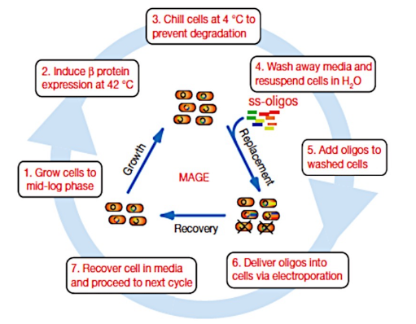
\includegraphics[width=0.5\textwidth, center ]{mage}
\caption{\label{fig:mage} MAGE automation}
\end{figure}
\noindent
To demonstrate an application of the MAGE process, they optimized metabolic flux through a biosynthesis pathway to overproducethe isoprenoid, lycopene, in an E. coli strain (EcHW2) that contained the pAC-LYC plasmid that is necessary for the final steps of lycopene production.
Specifically, for each of the 20 genes, 90-mer oligos containing degenerate ribosome binding site (RBS) sequences (DDRRRRRDDDD; D = A, G, T; R = A, G) flanked by homologous regions on each side were used, with a total pool complexity of 4.7 x 105.
Additionally, four genes (ytjC, fdhF, aceE, gdhA) from secondary pathways were targeted for inactivation by oligos that introduced
two nonsense mutations in the open reading frame, further improving flux through the DXP pathway.
Therefore, they optimized 24 genes simultaneously to maximize lycopene production.
As many as 15 billion genetic variants (4.3 x 108 bp variations per cycle for 35 MAGE cycles) were generated and screened (intense red pigmentation on Luria–Bertani agar plates).
Variants were isolated from 105 colonies screened after 5–35 cycles of MAGE and sequenced.
IWe have a huge variation in growth rate depending on the genetic background. We would expect a positive correlation between the mutation rate and growth rate,  but this is not straightforward.
For lycopene production in an E. coli strain, a 5 fold improvement in yield after three days was observed (pretty fast).
\\
\\
\noindent
On balance, MAGE is fast and efficient tuning of genetic diversity in E.coli. 
It may be applied to many MGE outcomes and ay be applicable to other organisms.

\section{CFPS and MAGE}
Goal: to test the Multiplex Automated Genome Engineering (MAGE) strategy to simultaneously modify and co-purify large protein complexes and pathways from the model organism Escherichia coli to reconstitute functional synthetic proteomes in vitro.
Ni-NTA Agarose is an affinity chromatography matrix for purifying recombinant proteins carrying a His tag. By adding 6 His tags on the C or N terminus on the protein of interest, we can isolate the full complement for the protein through affinity chromatography.
\\
\\
\noindent
In the study, nine total strainis were constructed for the ensemble PURE system.
Insertion of His-tag sequences into all target genes in the ePURE strains was characterized by PCR and subsequently verified by sequencing.
By application of over 110 MAGE cycles, they successfully inserted hexa-histidine sequences into 38 essential genes in vivo that encode for the entire translation machinery.
The colour codes are from four different population of cells. With this amount of changes, nothing managed to grow in the first population.  It was required to split into different sets, as the overall metabolic burden is too much.
